\section{Oszillatoren}
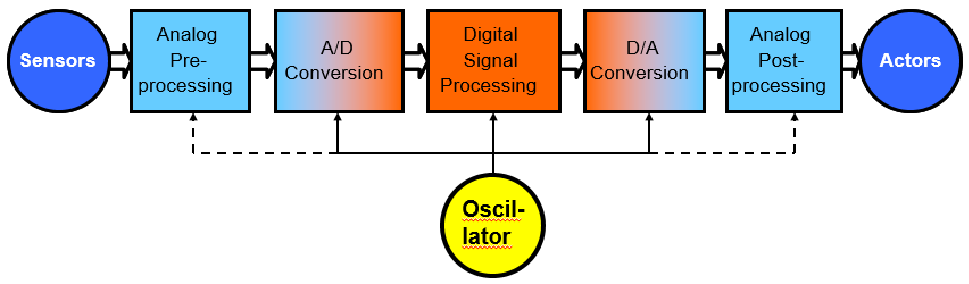
\includegraphics[width=\columnwidth]{images/oszi_overview.pdf}

\subsection{Klassifizierung}
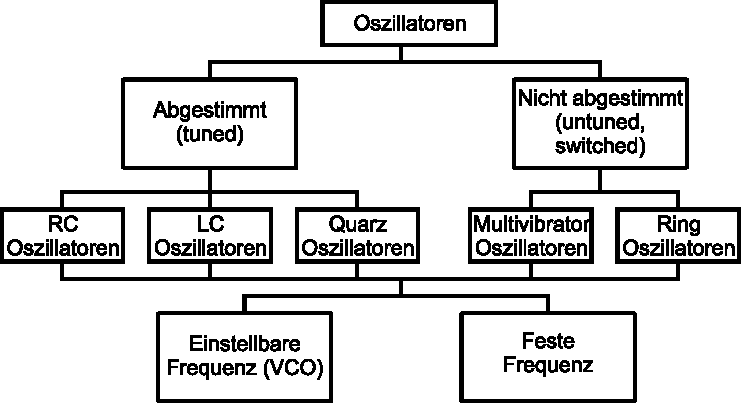
\includegraphics[width=\columnwidth]{images/oszi_klassifizierung.pdf}

\subsection{Scwingungsbedingungen}
Oszillatoren können gut als LTI-System dargestellt werden:

\begin{minipage}{0.34\columnwidth}
    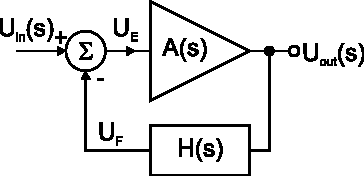
\includegraphics[width=\columnwidth]{images/oszi_system.pdf}
\end{minipage}
\hfill
\begin{minipage}{0.65\columnwidth}
    \begin{equation*}
        A_{CL}(s)
        = \frac{U_{out}(s)}{U_{in}(s)} 
        = \frac{A(s)}{1+A(s)H(s)} 
        = \frac{A(s)}{1+T(s)}
    \end{equation*}
    Folglich ist das Kriterium für eine Schwingung
    \begin{equation*}
        T(s) = -1
    \end{equation*}
\end{minipage}

Dabei wird der Input oft weggelassen, da dieser bei Oszillatoren nicht verwendet wird.
Entsprechend wird das Minus in eine der Übertragungsfunktionen geschoben:

\begin{minipage}{0.34\columnwidth}
    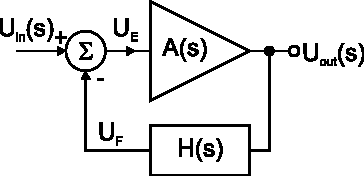
\includegraphics[width=\columnwidth]{images/oszi_system.pdf}
\end{minipage}
\hfill
\begin{minipage}{0.65\columnwidth} 
    \begin{equation*}
        A_{CL}(s)
        = \frac{U_{out}(s)}{U_{in}(s)} 
        = \frac{A(s)}{1-A'(s)H(s)} 
        = \frac{A(s)}{1-T'(s)}
    \end{equation*}
    Folglich ist das Kriterium für eine Schwingung
    \begin{equation*}
        T'(s) = 1
    \end{equation*}
\end{minipage}

\subsubsection{Frequenzstabilität}
\begin{minipage}{0.5\columnwidth}
    \input{figures/oszi_frequenzstabilität.tex}
\end{minipage}
\hfill
\begin{minipage}{0.49\columnwidth}
    Durch Einflüsse wie Störungen und Rauschen kann es sein, dass sich die Phase des Signals verschiebt.
    Eine grosse Phasensteilheit um die Resonanzfrequenz hilft dabei, den Einfluss dieser Phasenänderung auf die Frequenz zu minimieren.
\end{minipage}

\subsection{Amplitudenstabilisierung}
\begin{minipage}{0.5\columnwidth}
    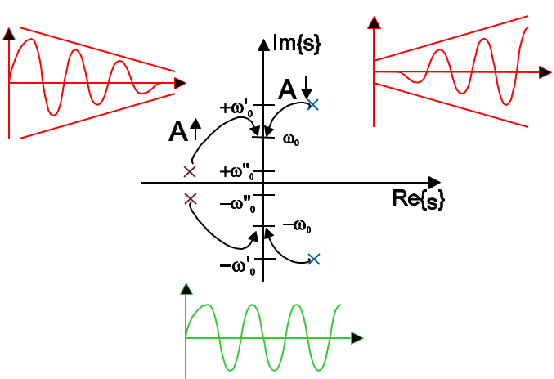
\includegraphics[width=\columnwidth]{images/oszi_amplitude.pdf}
\end{minipage}
\hfill
\begin{minipage}{0.49\columnwidth}
    Im Bild links ist der Zusammenhang zwischen Pollage und Amplitude gezeigt. 
    Liegen die Pole rechts der imaginären Achse, so nimmt die Ampliutde zu.
    Liegen sie Links, so nimmt die Amplitude ab. 
    Um die Amplitude konstant zu halten, müssen die Pole auf der imaginären Achse liegen.
\end{minipage}

\subsection{Mason}
Beim Evaluieren von OpAmp-Schaltungen werden oft die Übertragungsfunktionen mittels Mason ermittelt.
Deshalb hier nochmals die Masonsche Regel:

\begin{minipage}{0.4\columnwidth}
    \begin{equation*}
        H(s) = \frac{\sum G_k \Delta_k}{\Delta}
    \end{equation*}
    \begin{equation*}
        \Delta = 1 - \sum L_i + \sum L_i L_j - \cdots
    \end{equation*}
\end{minipage}
\hfill
\begin{minipage}{0.55\columnwidth}
    \begin{itemize}
        \item[$\Delta$:] Die Netzwerkdeterminante des Systems: 
            Eins minus alle Schleifen plus alle Produkte zweier Schleifen, die sich nicht berühren, minus \dots
        \item[$G_k$:] Das Gain des $k$-ten Forwärtspfads
        \item[$\Delta$:] Die Netzwerkdeterminante ohne alle Schleifen, die den Forwärtspfad berühren.
    \end{itemize}
\end{minipage}

\subsection{Abgestimmte Oszillatoren}
\subsubsection{LC-Oszillator}
Da der (Operations-) Verstärker bei LC-Oszillatoren nur die Verlustleistungen kompensieren muss, können LC-Oszillatoren effizienter als RC-Oszillatoren gebaut werden.

\textbf{OTA:}

\begin{minipage}{0.4\columnwidth}
    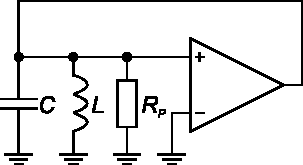
\includegraphics[width=\columnwidth]{images/oszi_ota.pdf}
\end{minipage}
\hfill
\begin{minipage}{0.55\columnwidth}
    Impedanz des Paralellschwingkreises:
    \begin{equation*}
        Z_{LCR}
        = \frac{1}{\frac{1}{s L} + \frac{1}{R_p}+s C}
        = \frac{L s}{C L s^2 + \frac{L}{R_p} s + 1}
    \end{equation*}
\end{minipage}
Mit der Übertragungsfunktion für einen Bandpass 2. Ordnung
\begin{equation*}
    H(s) 
    = \frac{\frac{A s}{\omega_0}}{\frac{1}{\omega_0^2} s^2 + \frac{1}{Q \omega_0} s + 1}
\quad \text{resultiert} \quad
    \omega_0 = \frac{1}{\sqrt{LC}} 
    \quad \text{und} \quad
    Q = \frac{R_p}{L\omega_0}.
\end{equation*}

\textbf{Mit OpAMP:}

\begin{minipage}{0.4\columnwidth}
    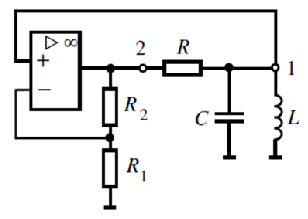
\includegraphics[width=\columnwidth]{images/oszi_opamp.pdf}
\end{minipage}
\hfill
\begin{minipage}{0.55\columnwidth}
    Die Übertragungsfunktion resultiert aus der Paralellschaltung der Reaktanzen und dem Widerstand $R$ als
    \begin{equation*}
        H(s) 
        = \frac{Z_{LC}}{R+Z_{lc}}
        = \frac{\frac{sL}{1+s^2LC}}{CLs^2 + }.
    \end{equation*}
    Wieder mit dem Koeffizientenvergleich resultiert
    \begin{equation*}
        \omega_0 = \frac{1}{\sqrt{LC}} 
        \quad \text{und} \quad
        Q = \frac{R_p}{L\omega_0}
    \end{equation*}
\end{minipage}

\subsubsection{Colpitts-Oszillator}
\begin{minipage}{0.4\columnwidth}
    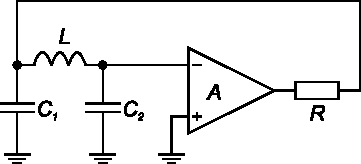
\includegraphics[width=\columnwidth]{images/oszi_colpitts.pdf}
\end{minipage}
\hfill
\begin{minipage}{0.55\columnwidth}
    Die Open-Loop Übertragungsfunktion $T(s)$ des Colpitts-Oszillators lautet
    \begin{equation*}
        T(s)
        = \frac{-A}{1+sR(C_1+C_2) + s^2 LC_2 + s^3RLC_1C_2}
    \end{equation*}
    Mit der Schwingungsbedingung $\Im(H(j\omega_0)) = 0$ sein muss, folgt
    \begin{multline*}
        j\omega_0 R(C_1+C_2) + {(j\omega_0)}^3 RLC_1C_2 
        = 0 \\
        \searrow \\
        \omega_0 
        = \frac{1}{\sqrt{L\frac{C_1 C_2}{C_1 + C_2}}}.
    \end{multline*}
\end{minipage}
Aus der Schwingungsbedingung $\Re(T(\omega_0)) = 1$ fürs Schwingen bzw. $\Re(T(\omega_0)) \geq 1$ fürs Anschwingen folgt
\begin{equation*}
    \Re(T(\omega_0))
    = \frac{-A}{1-\omega_0^2LC_2}
    \geq 1
\end{equation*}
und daraus
\begin{equation*}
    -A
    \geq 1 - \frac{C_1 + C_2}{C_1}
    \rightarrow
    A = \frac{C_2}{C_1}
    \quad \text{bzw.} \quad
    A \geq \frac{C_2}{C_1}
\end{equation*}
Die Übertragungsfunktion kann mittels Signalflussdiagramm und Mason relativ gut hergeleitet werden kann.

\subsubsection{Quarz-Oszillator}
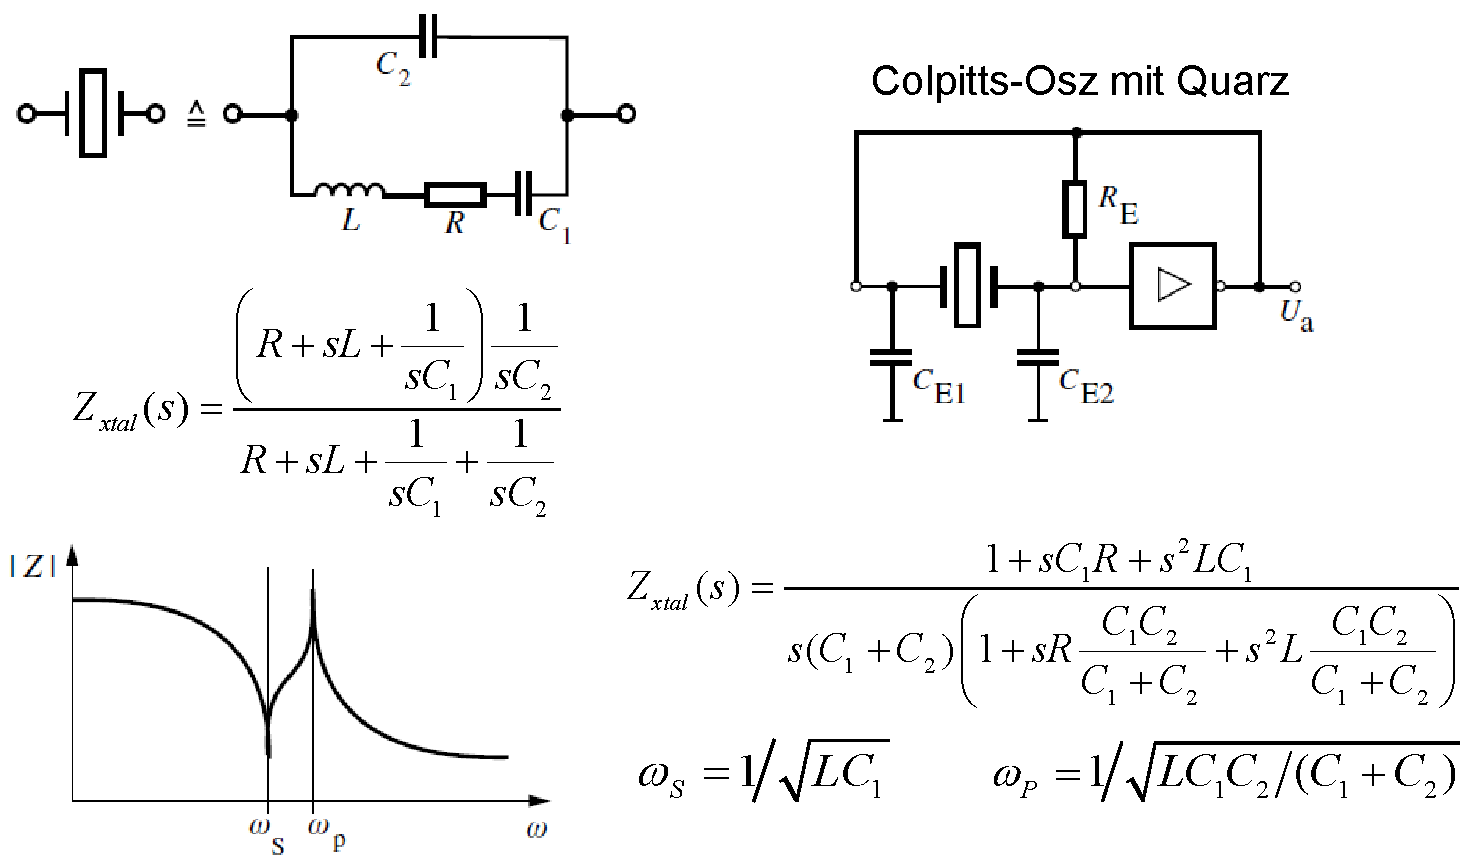
\includegraphics[width=\columnwidth]{images/oszi_quarz.pdf}

\textbf{Mit CMOS-Inverter:}

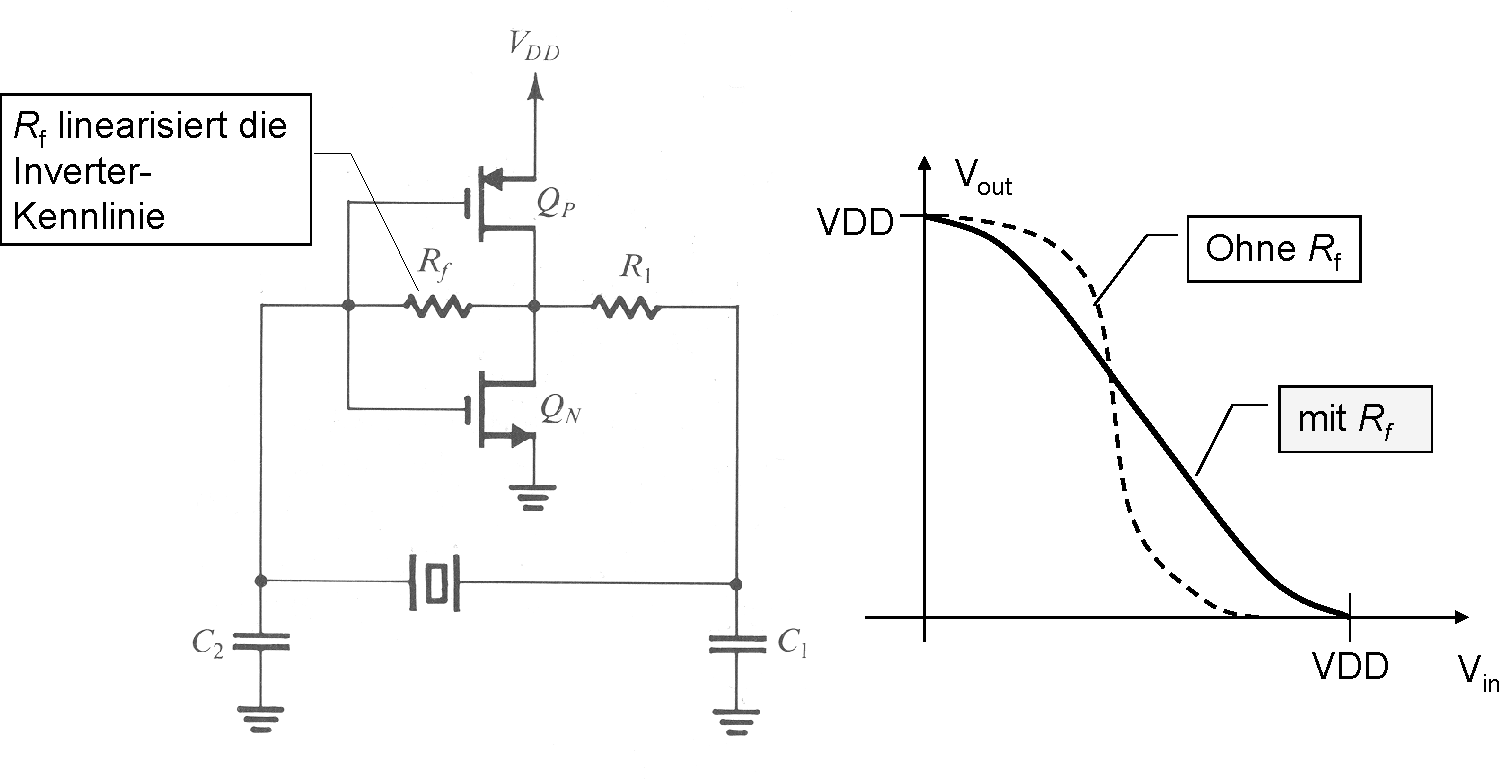
\includegraphics[width=\columnwidth]{images/oszi_quarz_cmos.pdf}

\textbf{Temperaturabhängigkeit:}

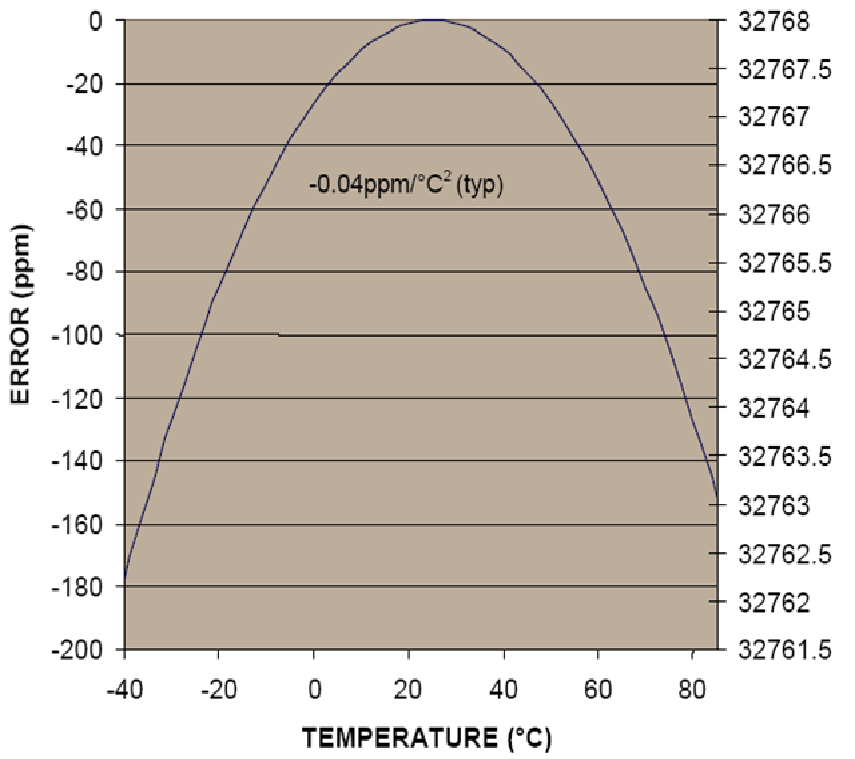
\includegraphics[width=\columnwidth]{images/oszi_quarz_temp.pdf}

\textbf{Quarz-Ersatzelemente:}

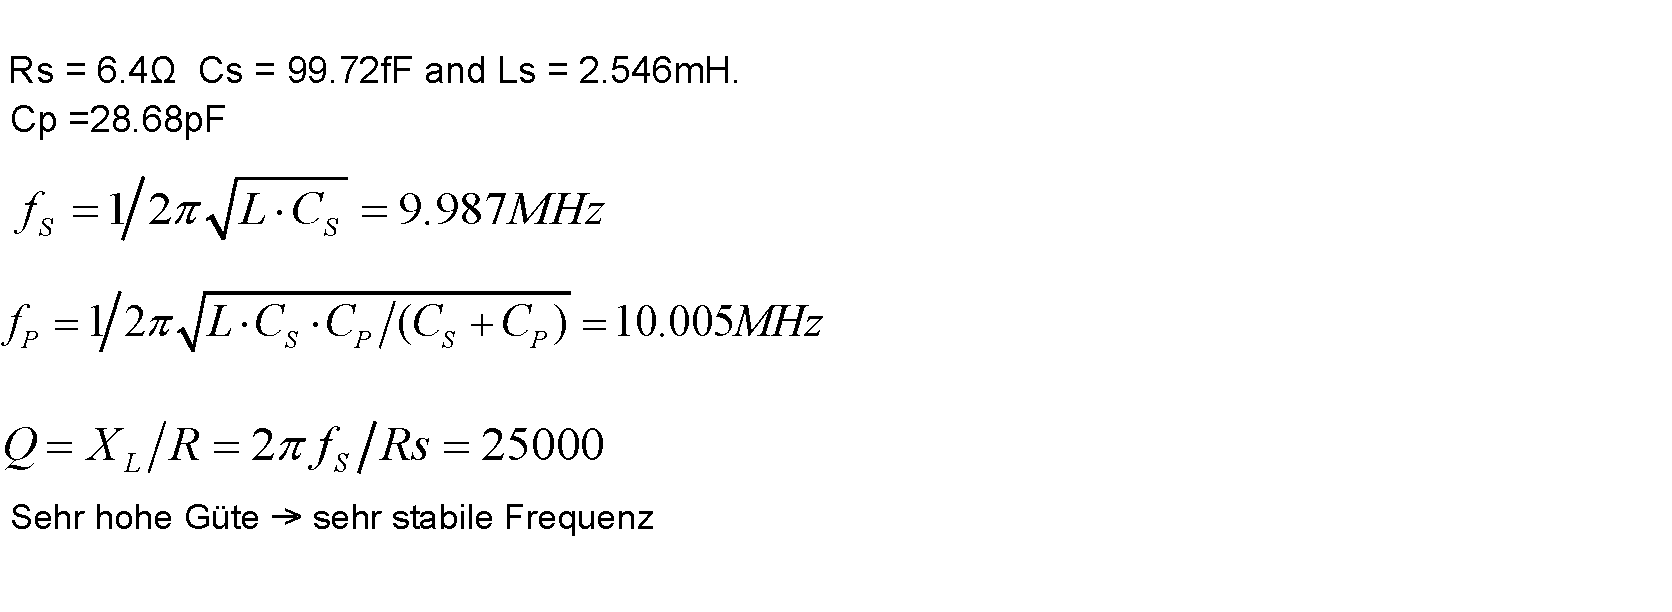
\includegraphics[width=\columnwidth]{images/oszi_quarz_bsp.pdf}

\subsubsection{Wien-Bridge}